\chapter{Guidelines and Best Practices for enhanced CLIP experiments and analysis}

\section{ABSTRACT}

Enhanced cross-linking immunoprecipitation (eCLIP) featuring a size-matched input control has been recently applied to profile the binding sites of more than one hundred RNA binding proteins (RBPs). However computational pipelines and quality control metrics needed to process CLIP data at scale have yet to be well defined. Here, we describe our ENCODE eCLIP processing pipeline (https://github.com/YeoLab/eclip), enabling users to go from raw reads to processed peaks that are enriched above paired input, reproducible across biological replicates, and can be directly compared against the public ENCODE eCLIP resource. In particular, we discuss processing steps designed to address common artifacts, including properly quantifying unique RNA fragments bound by both unique genomic- and repetitive element-mapped reads. Using manual quality annotation of 350 ENCODE eCLIP experiments, we develop metrics for quality assessment of eCLIP experiments prior to and after sequencing, including library yield, number of unique fragments in the library, total binding relative information, and biological reproducibility. In particular, we quantify the commonly believed linkage between depth of sequencing and peak discovery, and derive methods for estimating required sequencing depth based on pre-sequencing metrics. Finally we provide recommendations for the common question of integrating RBP binding information with RNA-seq to generate splicing maps representing the positional effect of binding on alternative splicing. These pipelines and QC metrics enable large-scale processing and analysis of eCLIP data, and will help to standardize rigorous analysis of RBP binding data.
 
\section{INTRODUCTION}
RNA binding proteins (RBPs) are major factors in the post-transcriptional regulation of gene expression. Recent estimates indicate that approximately 1,500 RBPs exist in the human genome\cite{Rutherford2008}. Collectively, these RBPs affect base modification, splicing, translation, nuclear export, subcellular localization, and stability of messenger RNAs, as well as processing of non-coding RNAs including microRNAs, ribosomal RNAs, and repetitive elements such as retrotransposons \cite{Bartel2004,Henras2015,Hung2015,Zarnack2013}. Manipulation of protein-RNA interactions is important in many aspects of human development, underscored by the identification of causal mutations in RBPs for diseases such as amyotrophic lateral sclerosis, fragile X syndrome, and cancers including medulloblastoma and chronic lymphocytic leukemia \cite{Daoud2009,Verkerk1991,Pugh2012,Wang2011}.

A critical first step in elucidating the function of RBPs is the identification of its RNA targets in vivo. Approaches such as UV crosslinking and immunoprecipitation followed by sequencing (CLIP-seq or HITS-CLIP) have enabled the transcriptome-wide discovery of RBP-RNA interactions at high resolution \cite{WAGENMAKERS1980,Greenberg1979,Ule2003}. These protein-RNA maps can reveal insights into the molecular roles of RBPs \cite{Yeo2009,Ule2003}. However, traditional CLIP-seq suffers from low ligation and crosslinking efficiencies, leading to poor experimental success rates and low reproducibility \cite{VanNostrand2016}. Variants of CLIP have addressed this in many ways, including increasing crosslinking efficiency with 4-thiouridine (PAR-CLIP) \cite{Hafner2010} and the incorporation of unique molecular identifiers (UMIs) to identify PCR duplicates (iCLIP) \cite{Konig2010}). Recently, enhanced CLIP (eCLIP) \cite{VanNostrand2016} and infrared-CLIP (ir-CLIP)\cite{Zarnegar2016} describe major improvements in the efficiency of generating sequencing libraries that led to dramatic increases in experimental success. This improved efficiency has enabled the incorporation of a paired size-matched input control experiment in eCLIP, which increases specificity in identifying high-confidence binding sites \cite{VanNostrand2016}. This approach has opened the door to large-scale profiling of RBP targets in vivo, enabling the ENCODE consortium’s efforts to profile 126 RBPs by eCLIP (Van Nostrand et al., in preparation).

With this considerable increase in the scale of eCLIP experimentation, there is a concomitant demand for improved methods to process eCLIP datasets and assess the quality of eCLIP datasets in an automated and scalable manner. Due to the variation in methodologies and low number of RBPs profiled in typical studies, current CLIP-seq quality control (QC) has traditionally been performed on a case-by-case basis, looking at individual binding locations \cite{Konig2010, Ule2003}, comparing results to known motifs \cite{Ray2013,Cook2011} or referring to previously published binding sites or known functions for the same RBP \cite{Weyn-Vanhentenryck2014,Zarnack2013}. Indeed, the first pass of quality scoring for ENCODE eCLIP datasets was performed by manual inspection \cite{VanNostrand2016}. However, these methods cannot often be performed for previously unstudied RBPs and do not scale, necessitating more structured metrics for the analysis of large-scale eCLIP datasets.

A similar requirement for robust, scalable quality metrics led the Chromatin ImmunoPrecipitation followed by sequencing (ChIP-seq) field to create a set of guidelines for sequencing depth, experimental design, and data quality. Including the use of Irreproducible Discovery Rate (IDR) analysis to determine reproducibility between biological replicates and provide highly confident and reproducible binding sites \cite{Li2011,Kharchenko2008,Jung2014}). These approaches were invaluable to standardizing the large-scale data generation performed as part of the ENCODE project and have become useful tools for the genomics community at large \cite{Dunham2012,Landt2012}. Strikingly, a re-analysis of public ChIP-seq data using these standards found that 20\% of published datasets were of low quality, confirming the value of such metrics in increasing robustness and reproducibility of trusted public datasets \cite{Marinov2013}.

Here we describe the development and implementation of data quality metrics and standards for eCLIP experiments performed as part of the ENCODE consortium efforts (Fig. 1A). Each of these datasets was manually assessed during data production, creating a reference set of high- and low-quality eCLIP experiments for proper evaluation of derived metrics. First, we developed experimental quality metrics to rigorously assay eCLIP experimental success prior to sequencing. Next, we developed a uniform processing pipeline to analyze 350 eCLIP datasets and evaluate the downstream effects of various processing choices \cite{VanNostrand2016}. Using these datasets, we derived effective computational quality control metrics to aid in analysis decisions. Finally, similarly to previous CLIP-seq pipelines \cite{Wang2014,Zhang2011,Uren2012,Althammer2011,Lovci2013,Corcoran2011}, we provide a portable set of eCLIP processing tools to reproduce data generated by the ENCODE project, process data newly generated data, and create ‘splicing maps’ of position-dependent regulatory activities. These tools and metrics will serve as a reference for future experiments within the ENCODE project and for the increasing number of other labs performing eCLIP.
 
\section{RESULTS}

\subsection{Experimental Quality Control Considerations}
The generation of high-quality, reliable RBP-RNA interaction datasets requires careful validation of two key experimental components: successful immunoprecipitation of the desired RBP, and successful library generation and sequencing. For these two components, we developed recommended metrics that enable rigorous validation of experimental success.

First, eCLIP experiments require the successful immunoprecipitation of a RBP of interest. This prerequisite requires the identification of a RBP-specific immunoprecipitation-grade antibody, which we previously addressed by screening over 700 antibodies to identify 438 “IP-grade” antibodies against 365 RBPs in K562 cells \cite{Sundararaman2016}. However, when we performed eCLIP we found that 18\% (54 out of 302) IP-grade antibodies failed to successfully immunoprecipitate the desired RBP in K562 cells (Supplemental Fig. S1A-B). This is perhaps unsurprising as eCLIP has numerous on-bead enzymatic steps and additional wash steps. Nevertheless this indicates that it is critical to perform an IP-western experiment as part of the standard eCLIP experimental protocol, as successful IP during eCLIP is not a given based on successful IP with other protocols. As such, we incorporated IP-western as a routine component of the eCLIP procedure, and IP-western images are provided for each ENCODE eCLIP experiment as part of the antibody metadata available at https://www.encodeproject.org.

A high-quality library is defined as one that is complex (i.e., it contains many unique RNA fragments relative to PCR duplicated fragments or other artifacts) and is critical for a successful eCLIP experiment. Thus, a quantitative metric for library complexity that can be applied prior to sequencing enables rapid culling of poor quality experiments and could help guide a desired sequencing depth by estimating an upper bound on the number of recovered RNA fragments. We previously introduced the extrapolated CT (eCT) metric that estimates the number of PCR cycles needed to obtain sufficient material for sequencing. This metric had appealing characteristics, as it was RBP-specific, showed high correlation with PCR duplication rate, and could be directly compared against eCLIP experiments performed with IgG isotype controls or antibodies in null cell lines \cite{VanNostrand2016,VanNostrand2017}.

However, we found that additional refinements were required to use eCT to derive recommendations for the optimal depth of sequencing. Although the initial eCT calculation assumed an idealized 2-fold amplification rate per PCR cycle, we observed that this rate is frequently lower in practice. To properly estimate PCR efficiency during eCLIP, we noted that at our standard sequencing depths some experiments had saturated the discovery of unique fragments, which enabled us to accurately estimate the total number of pre-PCR unique fragments for these datasets. Using 6 datasets with a PCR duplication rate of greater than 90\%, we observed that the best fit between the number of observed unique fragments, and the estimated number of unique fragments, occurred at a PCR efficiency of 1.84 (Supplemental Fig. S1C,D). We defined an accurate-eCT (a-eCT) as the eCT calculated with 1.84-fold amplification per cycle instead of 2-fold.

To validate the a-eCT metric, we considered datasets that were beginning to saturate (PCR duplication rate greater than 60\%). We observed that a-eCT showed strong predictive power for the number of unique RNA fragments observed ($R^2$ = .48, p $<$ 3.7e-38) (Fig. 1B), an improvement on the prior eCT metric (MSE 0.16 vs 0.82), confirming that a-eCT provides a robust estimate of library complexity (Supplemental Fig. S1E).

Next, we compared a-eCT against our manual annotation of experiment quality (Fig. 1A), and observed that experiments that pass manual quality assessment have a significantly lower a-eCT than experiments that failed manual quality assessment with mean a-eCTs of 13.2 vs 14.4 respectively (Fig. 1C, students t-test; p $<$ 10-7). Low a-eCT (corresponding to a highly complex library) did not always indicate high-quality eCLIP datasets, with failures due to poor reproducibility, lack of significant binding signal, and other failure modes (further discussed below). However, a high a-eCT value was a strong predictor of failure, typically due to a lack of the required number of unique fragments to produce reproducible binding regions. To establish a maximum a-eCT threshold beyond which data are unreliable, we observed that the mean a-eCT for IgG control eCLIP experiments (which only pull down background RNA) was 19.6. With that threshold applied, 18 out of 21 datasets with an a-eCT $>$ 19.6 also independently failed manual QC. In all datasets examined no successful experiment had an a-eCT > 20.7, while there were still 9 experiments that did not pass manual quality control that had a higher a-eCT (Fig. 1C).

In addition to providing a maximum cutoff for experiment quality, the strong predictive power among saturated datasets suggests that a-eCT can be used to estimate the total number of unique immunoprecipitated RNA fragments prior to sequencing (Fig. 1B). Considering all RBPs profiled, we observed a wide range of unique fragments from nearly 2 billion estimated for HNRNPU, to less than 320,000 for DROSHA (Fig. 1D). Thus, a-eCT can also be used to help guide desired sequencing depth, as high sequencing depth for samples with high a-eCT is essentially wasted sequencing of PCR duplicates (see further discussion below).


\begin{figure}[ht]
  \centering
  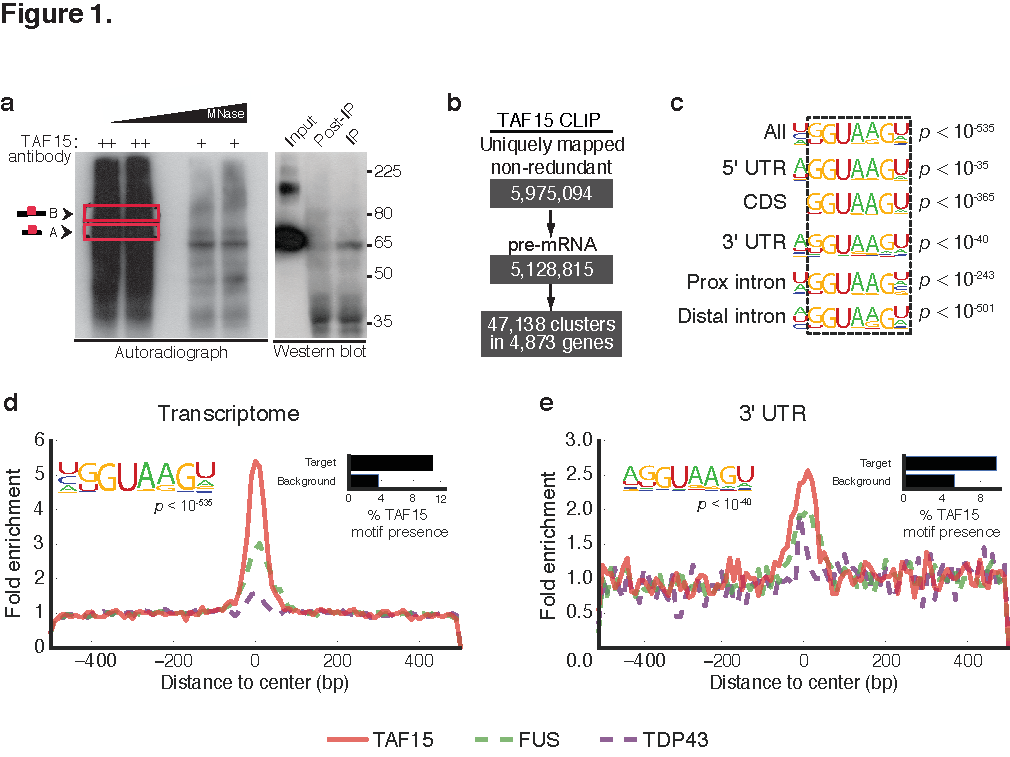
\includegraphics[width=0.5\textwidth]{chapter_3_figures/Figure_1}
  \caption[Figure 1. Estimation of unique RNA fragments recovered by a-eCT]{(A) Schematic of standard ENCODE experiment including manual quality control. (B) Scatter plot indicates accurate-eCT (a-eCT) (see Methods) versus unique fragments observed (including non-PCR duplicate reads mapped either to unique genomic loci or repetitive elements, in millions of reads mapped) for all ENCODE eCLIP experiments. Non-saturated ($<$60\% PCR duplicates) datasets are indicated in blue, and saturated ($>$60\% PCR duplicates) datasets are indicated in red. Dashed line indicates the number of unique molecules expected based on a-eCT. (C) Points indicate the a-eCT value of all ENCODE eCLIP experiments, separated into IgG controls (blue), datasets that failed manual quality assessment (red) and datasets passing manual assessment (green). Dotted line indicates average a-eCT of IgG control experiments (19.6). (D) Representative RBPs are listed along with their a-eCT and corresponding estimate of the number of unique RNA molecules isolated in eCLIP. UTP3 (in red) did not pass quality control metrics.\index{Figure_1}}
  \label{fig:Figure_1}
  \end{figure}

\begin{figure}[ht]
  \centering
  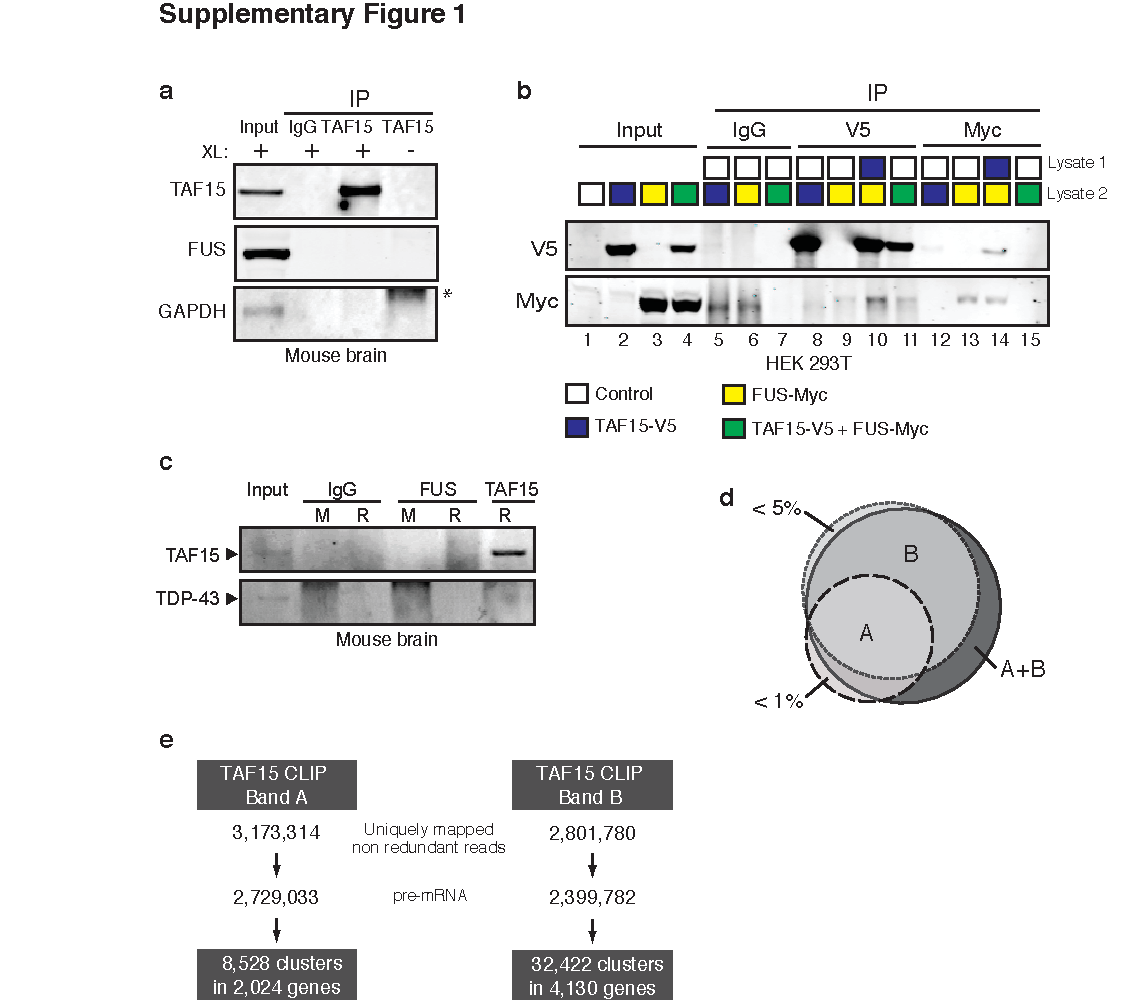
\includegraphics[width=0.5\textwidth]{chapter_3_figures/Figure_S1}
  \caption[Supplementary Figure 1. Estimation of unique RNA fragments recovered by a-eCT]{(A-B) Example immunoprecipitation (IP) western blots for proteins (A) DCP1B and (B) PES1 with successful IP using simplified conditions that exclude enzymatic library preparation steps, but failed to IP during full eCLIP. (C) Plot indicates sum of squared error for varying PCR efficiency when comparing true observed number of unique molecules to estimated number of unique molecules for six highly saturated ($>$90\% PCR duplicated) experiments. (D-E) Scatter plot of estimated unique molecules at two estimates of PCR efficiency, 2 (red) and 1.84 (blue) versus unique fragments obtained after sequencing. Shown are (D) six highly saturated ($>$90\% PCR duplicated) experiments, or (E) 255 moderately saturated experiments ($>$60\% PCR duplicated).\index{Figure_S1}}
  \label{fig:Figure_S1}
\end{figure}

\subsection{eCLIP Processing Pipeline}
Processing of raw eCLIP sequencing data is complex, as adapter sequences, double-adapter ligation products, retrotransposable elements and other multi-copy sequences, PCR duplicates, and underlying differences in RNA abundances all contribute to false negatives and false positives at both the read mapping and peak identification stages. To address these issues, we developed a rigorous standard eCLIP processing and analysis pipeline (Fig. 2A) \cite{VanNostrand2016}.

First, adapter sequences are aggressively trimmed to decrease potential false-negative mapping and to remove reads $<$18nt in length, which typically retains 91\% of sequenced reads (Fig. 1B). We observed that if adapter trimming is not performed correctly, the remaining adapter sequences often lead to mapping failures. To illustrate, 53\% of eCLIP fragments for the RBP RBFOX2 in HepG2 cells uniquely map to the genome if proper adapter trimming is performed, but only 35\% map if adapter trimming is not performed (Supplemental Fig. S2A).

Next, we considered repetitive elements and other multi-copy RNAs. These can represent true RBP associations: for RPS11 an average of 80\% of fragments mapped to repetitive elements including 68\% to the 18S rRNA, which is biologically consistent as RPS11 is a component of the 40S ribosomal subunit \cite{Taylor2009}. However, we observed that inclusion of these fragments in standard peak calling created significant artifacts, as these elements can have thousands of degenerate copies throughout the genome that lead to spurious peaks. For example, TIA1 and PTBP1 both bind the 3’ UTR of the MYADM mRNA, with enriched fragment density observed at a SINE element that is highly homologous to thousands of loci throughout the genome (Fig. 2C). If repetitive element fragments are not removed this SINE element is detected as a spurious peak between two authentic binding sites in both experiments (Fig. 2C). Thus, we developed two approaches: a standard peak calling and analysis approach that removes repeat-mapping fragments and only incorporates fragments that uniquely map to the genome, and another pipeline that quantitatively measures mapping to multi-copy element families (see below) (Fig. 2A). On average, 42\% of fragments were removed due to repetitive element mapping, and 33\% of sequenced fragments were uniquely mapped (with a standard deviation of 0.16 across 362 ENCODE eCLIP datasets passing manual quality control) (Fig. 2B). Although high, this variability is largely due to RBPs that associate with specific multi-copy RNAs (although we note that in cases of extremely low RNA yield, we have observed that bacterial RNA present in nitrocellulose membranes can contribute to the lack of mapping to the human genome) \cite{VanNostrand2017b}.

After mapping, PCR duplicate fragments are removed (using UMIs incorporated in library preparation prior to PCR amplification) to yield unique genomic fragments. An average of 66\% of unique genomic fragments remained after removal of PCR duplicates, although we observed an extreme range from 99.5\% of fragments remaining for hnRNPK in K562 cells to 4.6\% of fragments remaining for SF3B1 in K562 cells (Fig. 2B). We note that proper PCR duplicate removal is essential, as the presence of PCR duplicate reads can lead to regions of artificially high fragment coverage (often referred to as ‘skyscrapers’) that can be falsely identified as significant peaks, as in the case of hnRNPC (Fig. 2D). Overall, on average of 22\% of sequenced fragments remained after removing reads that were too short, non-uniquely mapping or PCR duplicates (Fig. 2B).

As multi-copy signals are not captured with our standard pipeline we developed an independent approach to quantify fragments that map to either multi-copy RNAs or unique genomic elements (Van Nostrand et al. in preparation). Datasets subjected to mapping to either repetitive or unique segments of the genome retained an average of 73\% of sequenced fragments for all RBPs, and were highly consistent, ranging from 71\% of sequenced fragments retained for SF3B1 in K562 to 85\% of sequenced fragments retained for CENPI in HepG2 (Fig. 2B). The fraction of PCR duplicate removed fragments was highly variable, with an average of 46\% of sequenced fragments retained after duplicate removal (see further discussion below) (Fig. 2B). In manual quality assessment of these datasets, we identify 25 experiments that did not pass based on standard analysis but were deemed high quality due to significant association to specific repetitive elements (Van Nostrand et al. in preparation).

Finally, significant peaks are identified using a two-step approach in which we first identify clusters enriched relative to local background, followed by input normalization. Input normalization is critical for the removal of common false-positive signals at abundant transcripts and enriches for motifs as well as RBP-responsive targets \cite{VanNostrand2016}. Cluster identification is performed using CLIPper, which uses spline-fitting to identify regions of enriched read density relative to both unspliced and spliced transcript-level background \cite{Lovci2013}. Reverse transcriptase enzymes will often terminate at the crosslinked nucleotide (due to amino acid adducts that remain after proteinase K treatment), which can be utilized to map crosslink sites with single-nucleotide resolution \cite{Konig2010}. As such, CLIPper was run using only the second, paired-end read in ENCODE eCLIP datasets, which is the read that begins at the putative site of reverse transcription termination. This yielded an average of 142,360 clusters per dataset, with a range from 647,011 clusters for hnRNPC in HepG2 to 1,910 clusters for SERBP1 in K562 (Fig. 2E). The read density within these regions is then compared in IP versus paired size-matched input to identify significantly enriched peaks \cite{VanNostrand2016}. We observed that a significant fraction (averaging 13\%) of clusters are depleted in IP relative to size-matched input, matching previous observations \cite{VanNostrand2016}. Applying a stringent threshold of requiring clusters to satisfy both fold-enrichment ≥ 8 and p ≤ 10-3 significance in IP versus size-matched input yielded an average of 7,146 high-confidence peaks, with a range from 48,173 peaks for PRPF8 in HepG2 to 43 peaks for AUH in HepG2 (Fig. 2E). On average, 6\% of clusters met this stringent threshold for enrichment (Fig. 2F). While we find that filtered clusters frequently fail both thresholds (an average of 68\% of clusters fail to meet both the fold-enrichment and significance threshold) (Supplemental Fig. S2B).

To identify reproducible and significantly enriched peaks across biological replicates, we used a modified Irreproducible Discovery Rate (IDR) method (Supplemental Fig. S2C). IDR requires that peaks are ranked by an appropriate metric, but we found undesirable results ranking peaks by either significance (due to the dependence on underlying expression) or fold-enrichment (due to the large variance of fold-enrichment when few reads are observed in input). Thus, we adapted relative entropy to better estimate the strength of binding in IP relative to input by defining the information content of a peak as $p_i*\log_2\frac{p_i}{q_i})$, where $p_i$ and $q_i$ are the fraction of total reads in IP and input respectively that map to $peak_i$. To confirm that this metric captures true binding signal, we considered the RBFOX2 eCLIP datasets. We observed 14,595 reproducible clusters when we ranked by fold enrichment, whereas 32,431 clusters were reproducible when we ranked by information content (Fig. S2D). Given the increased number of reproducible clusters detected, we used information content to perform standard IDR analysis to identify reproducibly bound regions \cite{Li2011}. We then identified the set of non-overlapping peaks from both replicates that maximized information content to define a final set of reproducibly enriched peaks that corresponded to CLIPper-identified regions (see Methods). This method revealed that an average of 53.1\% of peaks were identified as significantly enriched in individual replicates, confirming high reproducibility for most experiments (Fig. 2G).


\begin{figure}[ht]
  \centering
  \includegraphics[width=0.5\textwidth]{chapter_3_figures/Figure_2}
  \caption[Figure 2. Development of the eCLIP processing pipeline]{(A) Schematic of eCLIP processing for both unique genomic mapping and repetitive element mapping. (B) Points indicate the fraction of reads remaining after trimming (blue), mapping to either repetitive elements or unique segments of the genome (green), PCR duplicate removal on both repetitive elements and unique elements (red), mapping to only unique genomic elements (purple), and PCR duplicate removal on only unique genomic elements (yellow) for all ENCODE eCLIP experiments. (C) Effect of repetitive element masking on the gene MYADM. Tracks indicate raw read number for TIA1 (HepG2) and PTBP1 (HepG2) eCLIP datasets. Significant (fold-enrichment ≥ 8 and p-value ≤ 0.001) peaks are shown. SINE elements are derived from the RepeatMasker UCSC Genome browser track. The highlighted area indicates a peak overlapping a SINE element that is no longer detected after repetitive element removal. (D) Tracks indicate HNRNPC eCLIP read density in HepG2 in GPR126 for (top) without and (bottom) with PCR duplicate removal. Highlighted region represents ‘skyscraper’ that is lost during PCR duplicate removal. (E) Scatter plot of clusters versus significant peaks remaining after filtering (fold-enrichment ≥ 8 and p-value ≤ 0.001 in IP versus input). Histograms indicate cluster or peak distribution respectively. (F) Points indicate fraction of clusters meeting the above thresholds for p-value and fold-enrichment. (G) Plot indicates the number of significantly enriched peaks in replicate 1 of each eCLIP experiment versus the number of enriched and reproducible peaks in the total experiment after IDR analysis.\index{Figure_2}}
  \label{fig:Figure_2}
\end{figure}

\begin{figure}[ht]
  \centering
  \includegraphics[width=0.5\textwidth]{chapter_3_figures/Figure_S2}
  \caption[Supplementary Figure 2. Development of the eCLIP processing pipeline]{(A) Circles indicate fraction of reads effectively mapped in HepG2 RBFOX2 experiments if adapter trimming is not performed (blue), or is correctly performed (green) (B) Points indicate fraction of clusters removed due to specific filtering criteria, generally not enriched above input (red), enriched, but fail to meet p-value and fold change cutoff (blue), fails to meet only fold change cutoff (green) and fails to meet only p-value cutoff (purple) (C) Schematic of adaption of Irreproducible Discovery Rate (IDR) analysis to identification of reproducible eCLIP peaks. First, input-normalized clusters are identified separately for two biological replicates. Next, these peaks are ranked by relative information content, defined as $I_i=p_i*\log_2(\frac{p_i}{q_i})$, for proportion of IP reads within peak i represented by pi and fraction of input reads within the peak as qi. Next, standard IDR analysis is performed on the ranked peak lists to identify reproducible regions at IDR cutoff of 0.01. Next, we considered all CLIPper-identified subregions within these IDR regions, and calculated the fold-enrichment in IP versus input for each subregion in each replicate. Subregions were ranked by the geometric mean of fold-enrichment between the two replicates, and the set of non-overlapping subregions that were significantly enriched (p$<$0.001 in both replicates) with geometric mean of fold-enrichment ≥ 8 in both replicates were obtained as the set of reproducible peaks. (D) Plot indicates each peak ranked by IDR score, when IDR score is calculated by ranking peaks based on (blue) fold-enrichment above input or (green) information content.\index{Figure_S2}}
  \label{fig:Figure_S2}
\end{figure}


\subsection{Depth of sequencing does not significantly affect peak quality}
How deeply to sequence a CLIP-seq dataset is a major consideration (particularly at large scale), as samples must be sequenced sufficiently to robustly detect true binding signals while minimizing experimental cost. To develop recommendations for required sequencing depth, we considered two questions: first, how does sequencing depth affect identification of true binding sites, and second, how many reads are required to detect binding sites in any gene when accounting for variability in gene expression.

First, we asked whether peaks discovered at deeper sequencing depths were still likely to be biologically relevant. To do this we looked at RBFOX2, which is known to bind to the GCAUG motif. Overall, we observed significant enrichment for RBFOX2 binding to its motif, with 36\% of RBFOX2 peaks overlapping the motif vs a mean of 6\% of peaks overlapping the motif in all other datasets (Supplemental Fig. S3A). We then down-sampled the unique genomic fragments, re-called peaks, and asked how many peaks discovered at each down-sampling step overlapped the RBFOX2 motif. We observed that peaks discovered using only 10\% of unique genomic fragments showed the highest motif overlap (38\% on average), whereas peaks that were only discovered when going from 90\% to 100\% of unique genomic fragments were less likely to contain GCAUG (27\% on average) (Fig. 3A). Although this suggests that signal to noise is highest among the most abundantly covered peaks, we note that later discovered peaks were still 2.8- to 7.0-fold enriched above non-RBFOX2 datasets, indicating they still contain significant true binding signal (Fig. 3A). Supporting this, we observed that conservation of later-discovered peaks was similar to those discovered earlier with a mean phastcons conservation score of 0.136 versus 0.132 (Supplemental Fig. S3B). Considering an independent dataset, PRPF8, we observed similar results when testing its known association with the 5’ splice site: although peaks discovered at low sequencing depth were less enriched for true signal, we continued to see significant true positive signal throughout the range of down-sampling, indicating that it is true that deeper sequencing allows for the continued discovery of high quality peaks (Supplemental Fig. S3C, D).

Second, we considered the identification of binding sites as a function of sequencing depth. To explore if there was a correlation between sequencing depth and the discovery of peaks in lowly expressed genes, we calculated the correlation between gene expression and the number of reads in each peak for RBFOX2. We observed that lowly expressed genes had fewer reads per peak (as expected), whereas highly expressed genes displayed a large variation in the number of reads per peak, with only a weak correlation overall for both RBFOX2 ($R^2$ = .03) (Fig. 3B). All other RBPs showed a similar week correlation (mean $R^2$ = 0.24) (Supplemental Fig. S3E).

Next, we asked whether peaks at lowly expressed genes could be detected at standard sequencing depths. Surprisingly, we found that lowly expressed genes (defined as those with TPM $<$ 1) need on average only 870,000 unique genomic fragments to allow for detection of a peak in the gene, and this estimate was similar when varying the fraction of peaks required to be discovered or TPM thresholds (Fig. 3C, Supplemental Fig. S3F-H). As ENCODE eCLIP datasets have a mean sequencing depth of 4,509,000 unique genomic fragments, these results suggest that an inability to detect peaks on lowly expressed genes is not a major concern in eCLIP data sequenced to standard depths.

\begin{figure}[ht]
  \centering
  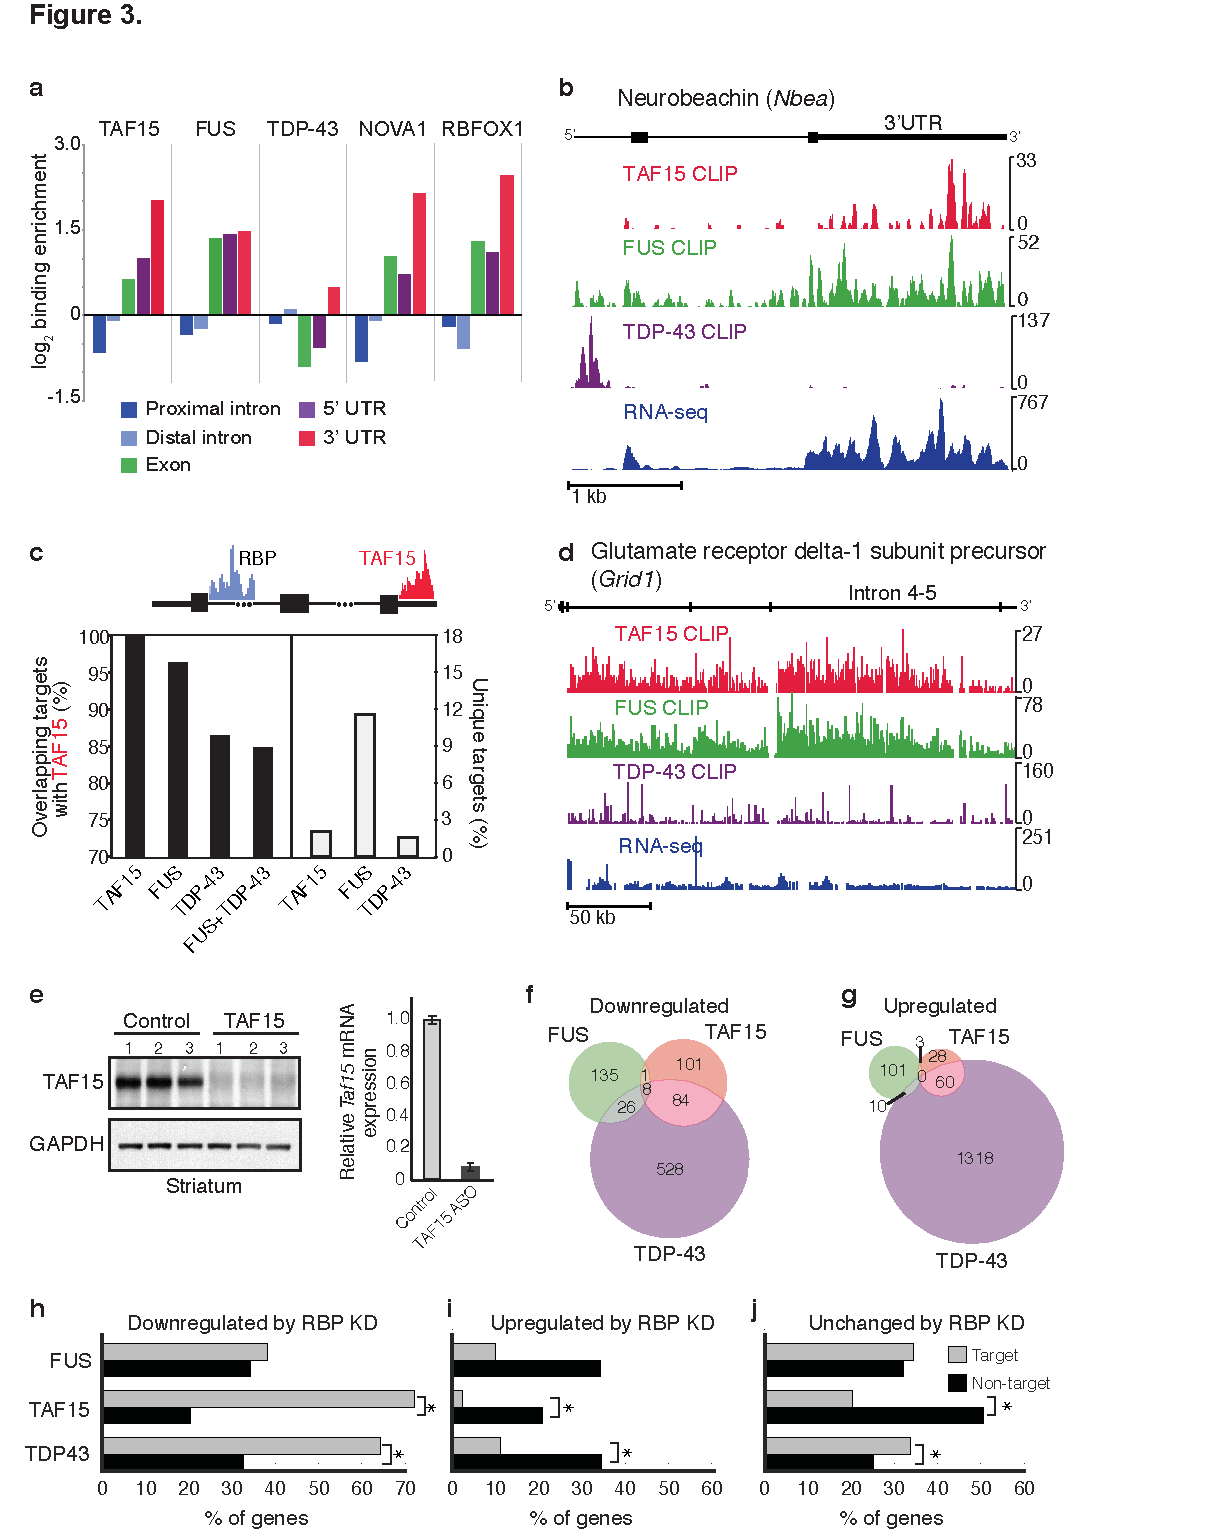
\includegraphics[width=0.5\textwidth]{chapter_3_figures/Figure_3}
  \caption[Figure 3. Dependency of peak discovery on sequencing depth]{(A) Plot of fraction of peaks containing a GCAUG motif for peaks identified in a series of subsamples of eCLIP unique genomic fragments for RBFOX2 in HepG2 and K562. Shown are RBFOX2 HepG2 replicate 1 (red) and replicate 2 (green), and RBFOX2 K562 replicate 1 (orange) and replicate 2 (blue). The dashed grey line indicates the mean fraction of GCAUG-containing peaks observed across all released eCLIP datasets. (B) One point for each gene indicates the TPM (Transcripts Per Million reads) of the gene (x-axis) and the number of reads (normalized by peak size) in the peak with the highest number of reads for RBFOX2 in HepG2. Dashed line indicates simple linear regression. (C) Joy plot indicates (top) the distribution of unique genomic fragment values for released ENCODE eCLIP experiments, versus (bottom) the distribution of total eCLIP unique genomic fragments in the downsampled subsample where the first peak was identified in each gene, separated into\index{Figure_3}}
  \label{fig:Figure_3}
\end{figure}

\begin{figure}[ht]
  \centering
  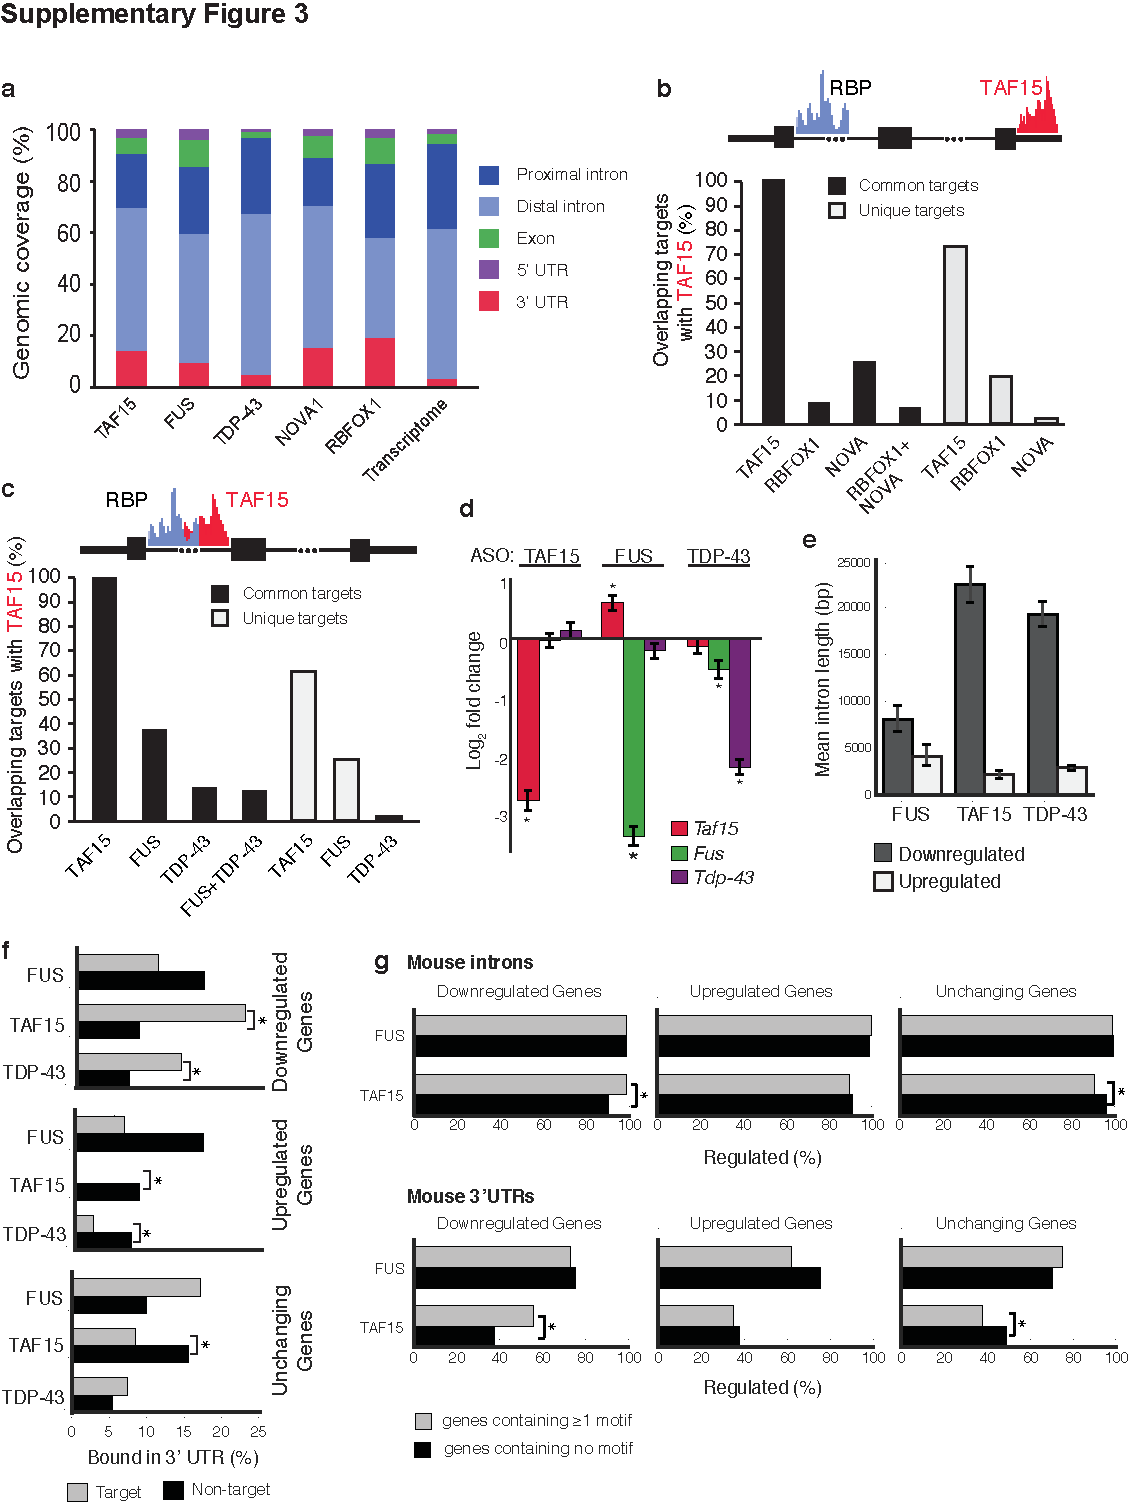
\includegraphics[width=0.5\textwidth]{chapter_3_figures/Figure_S3}
  \caption[Supplementary Figure 3. Dependency of peak discovery on sequencing depth]{(A) Points indicate fraction of significant peaks detected in between the 90\% to 100\% subsampled fraction that contain a GCAUG motif for all RBPs except RBFOX2 (blue) versus RBFOX2 (green) or fraction of all RBFOX2 peaks that contain GCAUG motif (red) (B) Plot indicates mean mammalian phastons conservation for all peaks newly discovered in each downsampled subsample for RBFOX2 eCLIP in HepG2 replicate 1 (red) and replicate 2 (green) and K562 replicate 1 (orange) and replicate 2 (blue). (C-D) Downsampling analysis for PRPF8 eCLIP in HepG2 replicate 1 (blue) and replicate 2 (green), and K562 replicate 1 (red) and replicate 2 (purple). (C) Plot indicates the fraction of peaks newly discovered in each downsampled subsample that overlap the 5’ splice site. The dashed grey line indicates mean fraction overlap with 5’ splice sites for all 179 non-PRPF8 released ENCODE datasets. (D) Lines indicate the average conservation for newly discovered peaks at the indicated downsampling fraction. (E) Points indicate the R2 (blue) and slope (green) for the linear regression between gene TPM and maximum peak read density for all released ENCOE eCLIP experiments. Each point represents an individual dataset as shown in Fig. 3B. (F) Density plot indicates the log10 number of reads in experiment (y-axis) when a gene with a specific log10 TPM is first detected to contain a peak (x-axis) for all released ENCODE eCLIP experiments. Green shading indicates the number of genes detected for each bin of read depth and TPM combination. The shaded region indicates number of reads needed to detect peaks when gene TPM $<$ 1. (left) Curve indicates the number of unique genomic fragments per released ENCODE eCLIP experiment. (G) Cumulative distribution function plot indicates the number of reads needed to first detect peaks for the set of genes in indicated bins separated by gene TPM: TPM $<$ .01 (blue), .01 ≤ TPM $<$ 1.0 (green), 1.0 ≤ TPM $<$ 10.0 (red), 10.0 ≤ TPM $<$ 100.0 (purple), 100.0 ≤ TPM (gold). (H) Plots indicate the cumulative fraction of genes with peaks discovered at given experimental sequencing depth, for the indicated cutoffs for peak enrichment in IP versus input (p-value ≤ .001 and fold-enrichment ≥ 8 (blue), p-value ≤ .01 and fold-enrichment ≥ 4 (green), p-value ≤ .05 and fold-enrichment ≥ 0 (red).\index{Figure_S3}}
  \label{fig:Figure_S3}
\end{figure}

\subsection{Saturation analysis suggests optimal sequencing depth}
Our analysis above indicates that continued sequencing until fragment saturation can recover true binding sites even at extremely high read depths. However, sequencing until fragment saturation is not typically economically reasonable. Thus, we set out to quantify diminishing returns upon deeper sequencing to identify the sequencing depth that optimally balances the tradeoff between gaining additional binding information and increased sequencing depth for an average eCLIP experiment (Fig. 4A).

First we developed a metric to quantify the diminishing returns of deeper sequencing in eCLIP datasets. Considering the discovery of significant peaks, we queried how many peaks were newly discovered when comparing peaks observed when 90\% or 100\% of fragments in a dataset were used to identify peaks. We observed that 71\% of experiments passing manual QC saturated the discovery of significant peaks (defined as the discovery of fewer than 5\% new peaks in the above metric), suggesting that simple peak detection was saturating for most but not all high-quality datasets (Fig. 4B).

We next considered whether binding information by total information content was saturating even when peak discovery was not. Summing the total information content across all peaks, we observed that information recovered saturated for 98\% of manually accepted datasets (using the same 5\% or less discovery metric between 90\% and 100\% of fragments used to call peaks in a dataset) (Fig. 4B). Thus, these results suggest that although additional peaks can be identified, the vast majority of binding information is already captured. We next asked at what sequencing depth total information content tends to saturate. We found that 90\% of all eCLIP datasets that passed manual quality assessment had saturated information discovery by 7.7M unique fragments (corresponding to 4.1M unique genomic fragments) (Fig. 4C, Supplemental Fig. S4A).

Next, we developed a model to estimate the number of sequenced reads that would typically be necessary to obtain the 7.7M suggested number of unique fragments. We observed that an average of 8.9\% and 4.7\% of reads are lost during adapter trimming and mapping, respectively (Fig. 2B). We also noted that when datasets are not near saturation (fraction usable $>$90\%) the PCR duplicate removal rate was on average 5.0\% (Supplemental Fig. S4B). Thus, in situations where there is a highly complex library, the number of unique fragments from sequenced reads can be estimated as $U=(1-P(a))(1-P(m))(1-P(d))*S$, where $U$ is the number of unique fragments, $S$ is the number of sequenced reads, and $P(a)$, $P(m)$, and $P(d)$ are the probabilities of losing a read due to adapter trimming, mapping and PCR duplicate removal, respectively. This model works well when datasets have a low PCR duplication rate (fraction usable $>$90\%) ($R^2$ = 0.91) (Supplemental Fig. S4C). However, because PCR duplicates often account for a large fraction of fragments lost, this method performs poorly when taking saturated datasets into account ($R^2$ = .55) (Supplemental Fig. S4C).

To address this limitation, we modeled PCR duplicate removal. Considering a pre-amplified library with E unique fragments PCR amplified to obtain a final library of ~100 femtomoles, we model the random sampling of individual reads as Poisson distributed. Specifically, the probability that a fragment is observed at least once can be calculated as $P(\leq1)=(1-e^{-\lambda})$, where $\lambda$ can be modeled as $\frac{M}{E}$ where $M$ represents the number mapped fragments and E represents the number of unique pre-amplified fragments (which can be estimated from a-eCT). Thus, the number of unique fragments $U$ obtained from $M$ mapped reads can be estimated as $U=E(1-e^{-(\frac{M}{E})})$ (Fig. 4D). This model predicted the actual number of unique fragments in each dataset with generally high accuracy (Fig. 4E, $R^2$ = .0.75). To further test this model, we compared the estimated number of unique fragments against the observed number of unique fragments identified in downsampling experiments as described above, and observed high correspondence for most datasets (median $R^2$ = 0.91) (Supplemental Fig. S4D). Thus, the Poisson model provides a highly accurate estimate for unique fragments obtained that is independent of sequencing and relies solely on the experimentally-obtained a-eCT.

Finally, merging the two above approaches allows us to back-calculate the number of sequencing reads S necessary to observe 7.7M unique fragments
$S=-E*\frac{ln(1-(U/E))}{P(a)P(m)}$. Using estimates for $P(a)$, $P(m)$ above yields final model $S=-E*\frac{\ln{1-\frac{7,700,000}{E}}}{0.868}$ where $E=\frac{100_{fm}*6.022*10^8_{\frac{molecules}{fm}}}{1.84^{aeCT}}$  (Fig. 4F). Considering the full range of a-eCT values, we observe that 10M fragments are sufficient for the majority of values, with slightly higher requirements for a-eCT values between 12 and 15 (Fig. 4G). Above a-eCT of 15 (where there are fewer than 7.7M estimated unique fragments in the pre-amplified library) we recommend targeting sequencing to observe 90\% of unique fragments (Fig. 4G, Supplemental Table S1). We find that the same depth of sequencing has proven sufficient for size-matched input experiments as well.


\begin{figure}[ht]
  \centering
  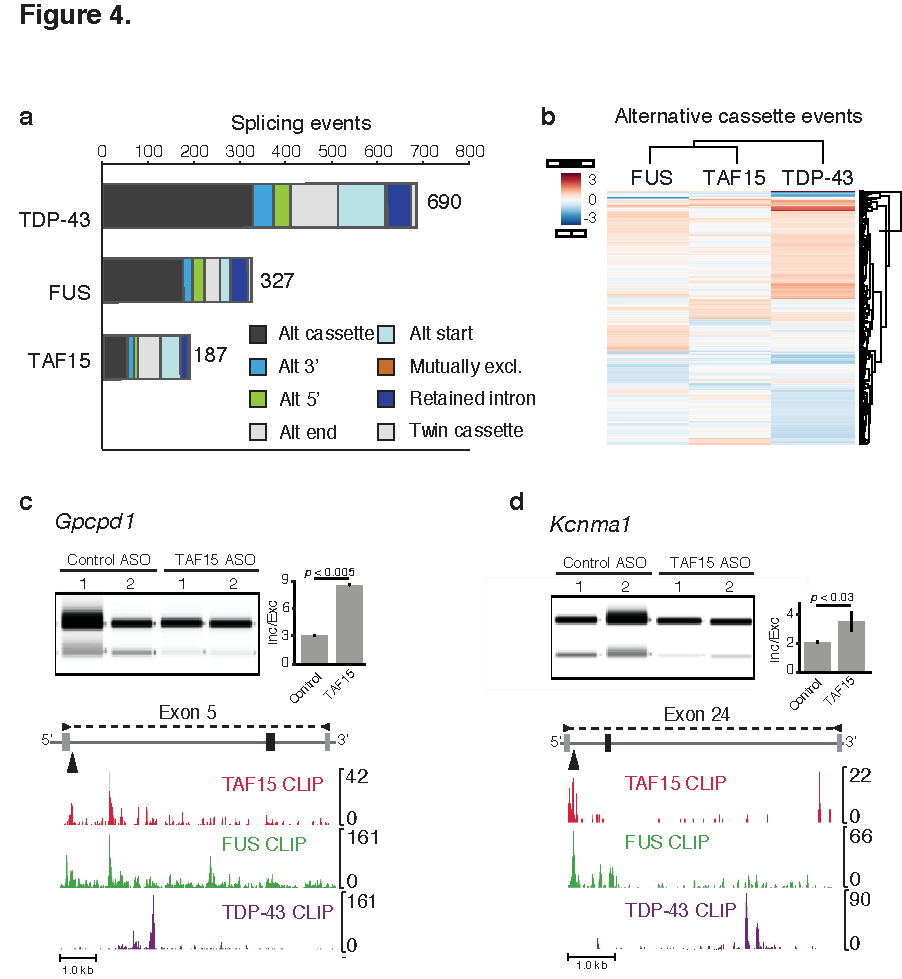
\includegraphics[width=0.5\textwidth]{chapter_3_figures/Figure_4}
  \caption[Figure 4. eCLIP Sequencing Depth Recommendations]{(A) Schematic of method used to estimate number of suggested reads for sequencing based on a-eCT calculation. (B) Points indicate saturation rate for peak or total information content between the 90\% retained and 100\% (full dataset) subsampled fraction for all submitted ENCODE eCLIP experiments. Grey dashed line is 5\% saturation cutoff. (C) (right) Lines show percent of additional information recovered when adding 10\% additional reads for hnRNPC (red), RBFOX2 (blue), and QKI (green) in HepG2. Dotted line indicates the ‘saturation’ point at which less that 5\% additional information is gained. (left) Cumulative fraction plot indicates the distribution of unique fragments when each eCLIP dataset reaches saturation. Colored points indicate depth of sequencing when hnRNPC, RBFOX2 and QKI saturate. (D) Plot indicates the relationship between mapped reads pre-PCR duplicate removal (x-axis) or unique fragments remaining post-PCR duplicate removal (y-axis) for actual downsampling experiments (green) or modeled using a Poisson estimate (red) for RBFOX2 in HepG2. (E) Scatter plot indicates observed versus estimated usable reads using Poisson model for all eCLIP datasets. (F) Schematic indicates how datasets with varying a-eCT values can be modeled to estimate required sequencing depth to obtain 7.7 million unique molecules. (G) Plot of a-eCT versus estimated number of input reads needed to obtain 7.7M unique molecules. For datasets with less than 7.7M estimated unique fragments (a-eCT $>$ 14.7), plot indicates the estimated number of reads to observe 90\% of total unique molecules (green). \index{Figure_4}}
  \label{fig:Figure_4}
\end{figure}

\begin{figure}[ht]
  \centering
  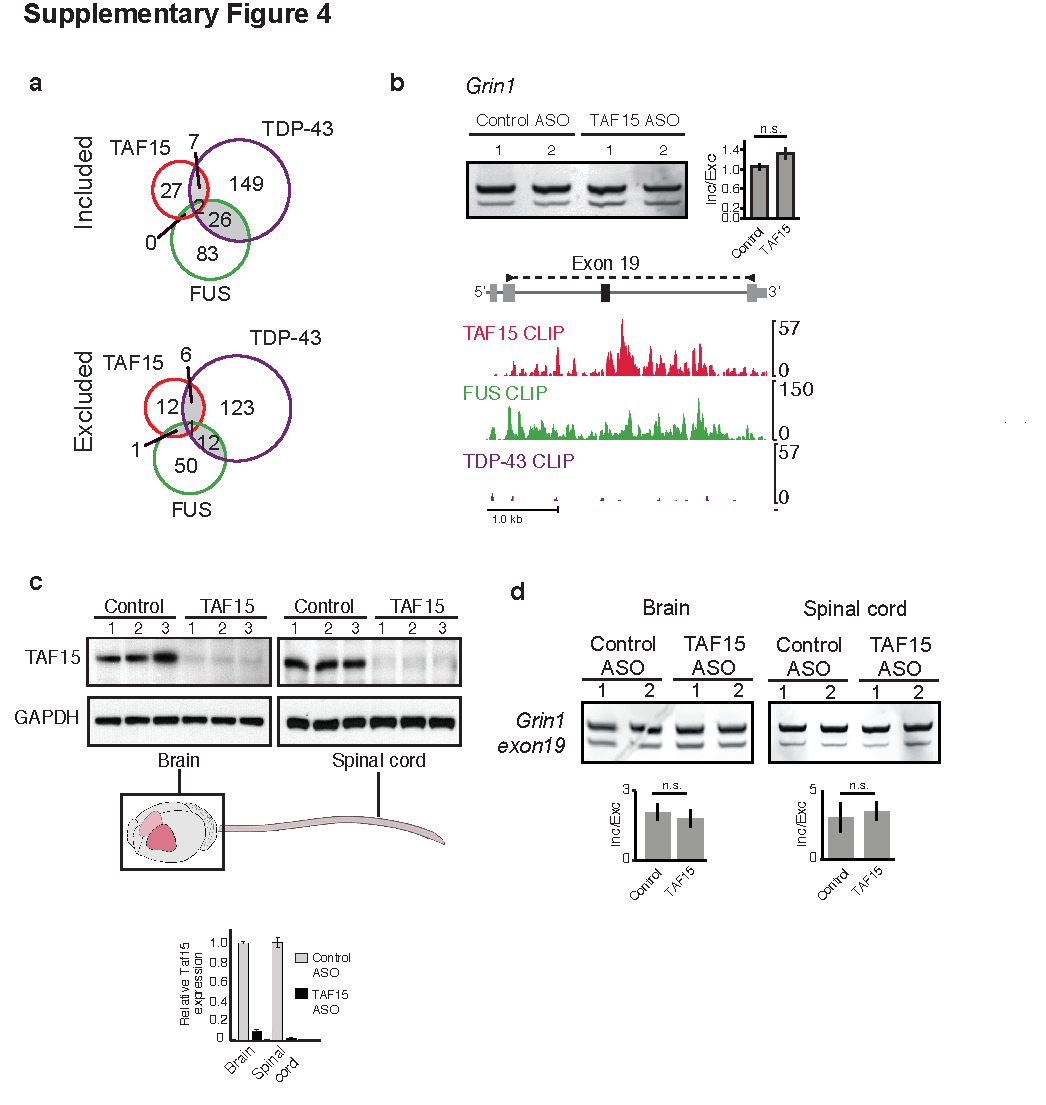
\includegraphics[width=0.5\textwidth]{chapter_3_figures/Figure_S4}
  \caption[Supplementary Figure 4. eCLIP Sequencing Depth Recommendations]{(A) Plot indicates the distribution of unique genomic fragments when each eCLIP dataset reaches saturation. Colored points indicate depth of sequencing when hnRNPC, RBFOX2 and QKI saturate. (B) Plot of fraction of unique fragments remaining after PCR duplicate removal is performed on mapped fragments in datasets with PCR duplicate rate of $<$10\% (C) Plot indicates (x-axis) the actual number of unique fragments versus (y-axis) the estimated number of unique reads using a naïve read estimation model with static fragment loss estimates for adapter trimming, mapping, and PCR duplicate removal. Shown are non-saturated (PCR duplication rate $<$ 10\%, blue) and all other datasets (red). (D) Histogram indicates R2 fits for all experiments using Poisson PCR duplicate read loss model (inset focuses R2 between 0 and 1). \index{Figure_S4}}
  \label{fig:Figure_S4}
\end{figure}

\subsection{Automated QC Metrics verify data quality}
We next developed a set of quality control metrics for ENCODE eCLIP experiments to assess the quality of individual datasets as well as the reproducibility across biological replicates (Fig. 5A). We ultimately arrived at two metrics for individual datasets: a minimal unique fragment cutoff, and a “total information in peaks” cutoff. To evaluate these metrics, we used manual quality assessment of datasets to define a reference set of high- and low-quality eCLIP datasets.

The number of unique fragments per dataset varies widely, depending on library complexity and sequencing depth (as described above). We observed that a required number of 1.5M unique fragments maximized the predictive power for datasets passing manual quality assessment (f-score = .86) (Supplemental Fig. S5A). Only 7 of 516 manually passed datasets do not meet this threshold: two (TBRG4, PABPC4) are not yet saturated and thus could be rescued by re-sequencing, whereas the 5 other datasets (one replicate of SLBP, two replicates of SF3B1, and SUPV3L1) are already highly saturated, but were considered high quality due to presence of signal at a small number of specific RNAs matching previous studies of these RBPs (histones, the U2 snRNP, and mitochondrial RNA respectively) (\cite{Townley-Tilson2006,Hodges1994,Borowski2013}. Conversely, 30 of 184 manually failed datasets do not meet the criteria (Fig. 5B). Thus, although the classification power of this model is low (AUC = 0.61), datasets not meeting this threshold were more than 16-fold more likely to fail manual quality assessment (Supplemental Fig. S5B).

Next, we considered a metric based on whether the dataset contained significant binding signal. As described above, we observed that the relative information of a peak better captures the binding information of peaks across genes with widely varying expression levels. Thus, to validate that a dataset contains significant binding information, we calculated the sum of relative information across all peaks in the dataset. We observed that this total information content score maximized the f-score of manually annotated high- and low-quality datasets at a total information content of .044 (f-score = .89) (Fig. 5C, Supplemental Fig. S5C). The information content model was highly accurate (AUC = 0.75), accurately classifying 77\% of ENCODE datasets with 0.48 specificity and 0.92 sensitivity (Supplemental Fig. S5D).

Next, we developed criteria to assay biological reproducibility, using two metrics based upon the Irreproducible Discovery Rate (IDR) approach that has previously been used to assay reproducibility of ChIP-seq peaks: reproducibility between real and pseudo-replicates (Rescue Ratio) (Supplemental Fig. S5E) and confirmation that the number of reproducible peaks between both replicates is similar (Self-Consistency Ratio) (Supplemental Fig. S5F) (Landt et al. 2012). We found that cutoffs previously used for ChIP-seq data could be similarly applied to eCLIP \cite{Landt2012}, and observed that 81.4\% of experiments have a passing rescue ratio of $<$2 (Supplemental Fig. S5G) and 70\% of experiments have a passing self-constancy ratio of $<$2 (Supplemental Fig. S5H). 221 experiments pass both thresholds, while 89 are borderline (passing one of the two thresholds), and 40 fail both thresholds (Supplemental Fig. S5I). Notably, these IDR metrics have high specificity, as 180 out of 221 (79\%) of experiments that meet unique fragment and total information content cutoffs and were manually judged to be high quality passed this IDR critera. In contrast, IDR detects potential false positives by correctly failing 9 out of 28 (32\%) datasets that met read depth and information content metrics, but failed manual inspection (Fig. 5D).

Finally, we combined these metrics into one overall automated quality call requiring that each experiment passes minimum read and entropy cutoffs as well as either being classified as passing or borderline based on IDR metrics (Fig. 5E). Overall our model accurately classified 83\% of eCLIP datasets with a sensitivity of 0.84 and a specificity of 0.79 (Fig. 5F), better than any individual classification scheme.


\begin{figure}[ht]
  \centering
  \includegraphics[width=0.5\textwidth]{chapter_3_figures/Figure_5}
  \caption[Figure 5. QC Guidelines for paired eCLIP experiments]{(A) Schematic of eCLIP data quality standards. (B) Swarm plot indicates number of unique fragments observed in each eCLIP dataset separated by failing (red) or passing (green) manual quality inspection. Dashed line indicates 1.5 million read quality threshold that maximizes predictive power on manual classification (Supplemental Fig. 5A), and inset indicates confusion matrix for this threshold versus manual inspection. Three datasets judged to be high quality despite low unique fragment number are indicated. (C) Similar swarm plot indicates the total information content across all peaks in each eCLIP dataset that passes the unique fragment threshold in (B), separated by failing (red) or passing (green) manual quality inspection. Dashed line indicates the information content threshold that maximizes predictive power on manual classification (Supplemental Fig. 5C), and inset indicates confusion matrix for this threshold versus manual inspection. (D) Bar chart indicates the count of all ENCODE experiments that pass or fail manual or automated QC approaches, broken into three groups based on their IDR thresholding metric status: passed (blue), borderline (green), and failed (red). (E) Schematic detailing final recommended quality assessment decision flowchart. (F) Confusion matrix of final classification scheme versus manual quality assessment.\index{Figure_5}}
  \label{fig:Figure_5}
\end{figure}

\begin{figure}[ht]
  \centering
  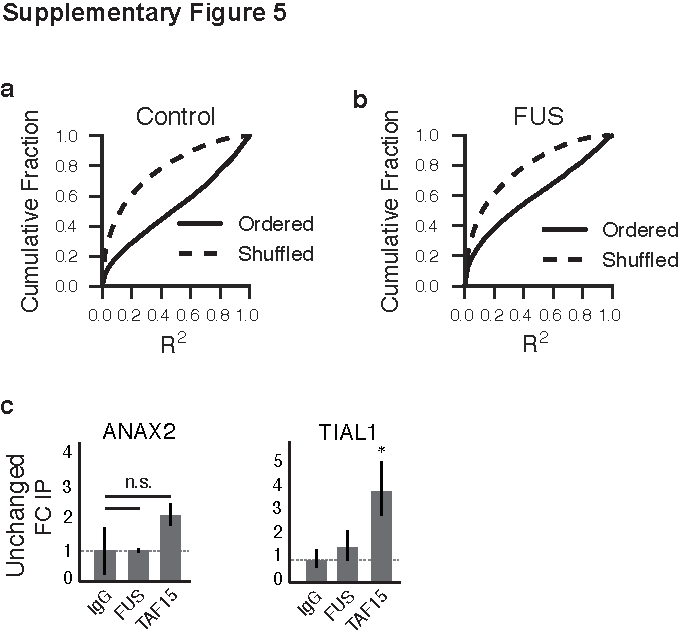
\includegraphics[width=0.5\textwidth]{chapter_3_figures/Figure_S5}
  \caption[Supplementary Figure 5. QC Guidelines for paired eCLIP experiments]{(A) Plot indicates f-score for classification of datasets relative to manual quality assessment based on unique fragments present. Maximal classification of datasets was obtained at a cutoff of 1.5 million unique fragments. (B) ROC curve for classifying datasets based upon varying minimum unique fragment thresholds. (C) Plot indicates f-score for classification of datasets based on the total information content in all significantly enriched peaks. Only datasets passing the unique fragment cutoff in (A) were considered. (D) ROC curve for classifying datasets based upon varying total information in peak cutoff. (E) Schematic for calculation of Irreproducible Discovery Rate rescue ratio. (F) Schematic for calculation of IDR self-consistency ratio. (G) Bar plot indicates rescue ratio for all ENCODE eCLIP experiments. (H) Bar plot indicates self-consistency ratio for all ENCODE eCLIP experiments. Dashed line indicates a cutoff of 2 previously used for ChIP-seq analysis. (I) Bars indicate the number of ENCODE eCLIP experiments that either pass both rescue ratio and self-consistency ratio (pass, blue), passed just one of the two tests (borderline, green) or failed both tests (fail, red).\index{Figure_S5}}
  \label{fig:Figure_S5}
\end{figure}

\subsection{eCLIP Pipeline Implementation}
We previously described the implementation of our eCLIP processing pipeline \cite{VanNostrand2016}. However, implementation of the pipeline is non-trivial, and difficult to reproduce in other computational environments. To address the problem we have made available a reference version of the pipeline runs locally on a cluster through a pipeline definition in Common Workflow Language (CWL). Our eCLIP processing pipeline handles fastq demultiplexing, PCR duplicate removal and peak calling including input normalization (Fig. S6A). Additionally, we produce an automated quality control report, describing the metrics developed throughout the paper. A major advantage to this structure is to both simplify and standardize the definition of all associated metadata, which is now explicitly structured in a single input manifest. Key output files match those deposited at the ENCODE Data Coordination Center, and include mapped reads (in compressed bam format), and identified clusters and significant peaks (in bed format). Due to being created with CWL this pipeline is highly portable, able to run on any mac or Linux installation with minimal effort. 

\begin{figure}[ht]
  \centering
  \includegraphics[width=0.5\textwidth]{chapter_3_figures/Figure_S6}
  \caption[Supplementary Figure 5. CWL Pipeline Design]{Schematic of eCLIP CWL processing pipeline\index{Figure_S5}}
  \label{fig:Figure_S6}
\end{figure}

\subsection{Integration of eCLIP with RNA-seq to generate regulatory maps}
Once direct binding sites are identified with eCLIP or related methods, it is common to integrate this information with independent datasets (such as transcriptome profiling upon RBP knockdown or over-expression) to gain insight into which interactions drive differential regulation of the bound transcript. This has proven particularly insightful for regulation of splicing, where RBP binding can cause either inclusion or exclusion of alternative exons depending on whether binding occurs in the upstream or downstream intron \cite{Yeo2009}. This location-dependent splicing regulation is often visualized as a ‘splicing map’, and the generation of splicing maps for different RBPs has become an important visualization tool to provide mechanistic hints into the global regulation of alternative splicing by RNA binding proteins. However, we observed that multiple decision points regarding integration of eCLIP data into the splicing map, for example using either read density or peaks (each of which can be normalized in various ways) can yield significantly different maps \cite{Witten2011,Huelga2012}. The scale of data generated here enabled us to query the effects of these choices across multiple datasets.

The first decision regards what events to consider in a splicing map. For visualization purposes, only a meta event is shown - for example, cassette exon events (the most commonly visualized splicing maps) are represented as a three exon region to show the upstream splice site, the 5’ and 3’ splice sites of the cassette exon, and the downstream splice site, although analogous approaches can be used to visualize alternative 5’ and 3’ splice sites or retained intron events (Fig. 6A, top). A set of exons is then defined to build the map, typically based off of a set of RBP-responsive events that show significant splicing alteration upon RBP knockdown or over-expression. In generating these sets of exons, we noted that it was common for splicing analysis pipelines to identify overlapping alternative exons. However, if two or more skipped events overlap at any position, these positions become susceptible to integrating the same CLIP signal multiple times (Supplemental Fig. S7A). To avoid this, we conservatively group overlapping events and select only those with the highest inclusion junction count. We found that standard differential splicing analysis tools yielded an average of 20\% overlapping events, indicating that this can represent a significant artifact if not considered (Supplemental Fig. S7B).

Next, we explored options for incorporating eCLIP data. First, we considered splicing maps built off of density of significantly enriched peaks \cite{Huelga2012}. These maps are typically simplest to calculate, as peak density over the meta region is simply summed across all events. We found that this approach yielded clear maps for RBPs such as RBFOX2 with a large number of bound differential events (Supplemental Fig. S7C). However, the main drawback of this approach is limited power, as the mean number of peaks covering a skipped exon region in a ENCODE datasets is only 31 (Supplemental Fig. S7D). Indeed, for SRSF9, a map made using read density shows enrichment at events excluded upon SRSF9 knockdown; however, because there are only 4 peaks overlapping skipped exon regions, peak based analysis shows no significant sites (Fig. 6A).

We hypothesized that incorporating read density instead of simply peak location could improve splicing map power. Considering eCLIP data, we first noted that traditional splicing maps built on iCLIP and CLIP data do not contain normalization against a paired input \cite{Konig2010}. We observed that this approach could be applied to eCLIP data for RBPs such as HNRNPK that already have high signal-to-noise, where the map showed a significant enrichment for binding signal at exons included upon knockdown that recapitulates the general repressive role for HNRNP proteins (Fig. 6B, Supplemental Fig. S7E). However, we noted that if one generated a splicing map from input alone, there exists significant variation in binding density (with particular enrichment of signal at exons in general) (Fig. 6C, Supplemental Fig. S7F), suggesting that input normalization could improve signal-to-noise in identifying regions enriched above background.

To explore input normalization within CLIP density maps, we applied two normalization strategies: background subtraction and information content-based normalization (Fig. 6D). Background subtraction first normalizes the binding density across each event, and then subtracts the input density from a corresponding IP experiment. In this case, the binding profile at event is weighted equally, resulting in a map that reflects the global shape of binding at the cost of muting regions with signal from a small number of events (Fig. 6E, Supplemental Fig. S7G). As an alternative approach, we calculated the relative information (in IP versus input) at each position for each queried event. The distribution across all events is then used to create the splicing map (using the mean and standard error calculated across all events for each position). As relative information is dependent on abundance, in this approach more abundant binding events will contribute more to the overall splicing map, events with high input, and low IP abundances contribute less strongly to reduction in overall signal, which can be a desired property in some cases (Fig. 6F, Supplemental Fig. S7H-J).

In both cases, we observed that individual highly abundant positions at single events could dominate the composite signal. Manual inspection suggested that these often arise from miRNAs, pseudogenes, and other multi-copy or highly abundant transcripts present within these intronic regions. To address this, we performed outlier removal on the top and bottom 2.5\% signal at each position across the splicing map. For example, we observed a site of significant enrichment approximately 250bp downstream of knockdown-excluded skipped exons for HNRNPC. However, after removing a single outlier element, the HNRNPC splicing map shows primarily 3’ splice site and exonic signal at exons included upon knockdown, consistent with the splicing-repressive role of HNRNP proteins (Fig. 6G, Supplemental Fig. S7K-L)

Finally we explore the utility of utilizing CLIP crosslink-diagnostic events that allow for the detection of the exact theoretically crosslinking site \cite{Rossbach2014, Konig2010}. For the previous analyses, we calculated read density by including bases covered by the entire read. However, reverse transcription often terminates at the site of protein-RNA crosslinking, which causes the 5’ end of reads to often correspond to the site of RBP-RNA interaction (with some variability due to the positioning of available crosslinkable amino acids and bases within the binding site) \cite{Konig2010}. When we queried how using only the 5’ end of reads could affect splicing map signal and noise, we observed that the effect was heavily dependent on different RBPs. For some RBPs such as U2AF2, we observed that the use of only the 5’ end of reads provided significant clarity to the splicing map by resolving binding to specific regions (for example, in U2AFC the intronic 3’ splice site region is enriched as opposed part of the alternative exon) (Fig. 6H, Supplemental Fig. S7M). However, for other RBPs such as RBFOX2 we observed that using 5’ read ends yielded a similar map, but with dramatically increased noise relative to using whole reads (Supplemental Fig. S7N). Thus, these results suggest that this method can improve resolution for some RBPs (particularly those with highly specific splice site-proximal binding), but that factors with broader crosslinking and binding patterns may suffer unacceptable loss of signal.

\begin{figure}[ht]
  \centering
  \includegraphics[width=0.5\textwidth]{chapter_3_figures/Figure_6}
  \caption[Figure 6. Considerations for design of splicing maps]{(A) (top) Schematic of cassette exon splicing. (bottom) Comparison of splicing maps generated for SRSF9 (HepG2) knockdown-excluded cassette exons based on peak (blue), background subtracted normalized read (gold) or non-changing background read (black) density. Bars above plot indicate areas of significant enrichment (by Mann-Whitney U test) above background when either peaks or reads are used. (B) Splicing map for HNRNPK (HepG2) binding at knockdown-included (red) or native (black) events generated from read density in IP. The region shown includes 300 nucleotides of intronic sequence upstream or downstream of the skipped exon, and 50bp of exonic sequence on both the 5’ and 3’ sides. Boxes indicate regions discussed in the text. (C) As in (B), but showing read density in input. (D) Schematic shows calculation of background subtraction and entropy normalization methods. (top) For background subtraction, read coverage is first normalized within each event by dividing each position by the total read coverage. Input signal is then subtracted from IP signal to create a map for each event. Final splicing maps represent the mean across all events. (bottom) Read density within events is first normalized for overall sequencing depth. Then relative information is calculated at each position to yield an event-level map. All events are then averaged to yield the final splicing map. (E) Similar to (B), plot shows the background subtraction splicing map for hnRNPK. (F) Similar to (B), plot shows the information content splicing map for hnRNPK. (G) Effect of removing outliers (defined as the 2.5\% of the top and bottom most enriched elements at each position). Plot indicates mean information content normalized density before (dark red) and after (light red) removing outliers. (H) (top) Schematic of whole read (orange) versus 5’ end (green) read coverage. (bottom) plot indicates U2F2 eCLIP mean background subtracted normalized read density at cassette exon 3’ splice sites for U2AF2 knockdown-included events in HepG2.\index{Figure_6}}
  \label{fig:Figure_6}
\end{figure}

\begin{figure}[ht]
  \centering
  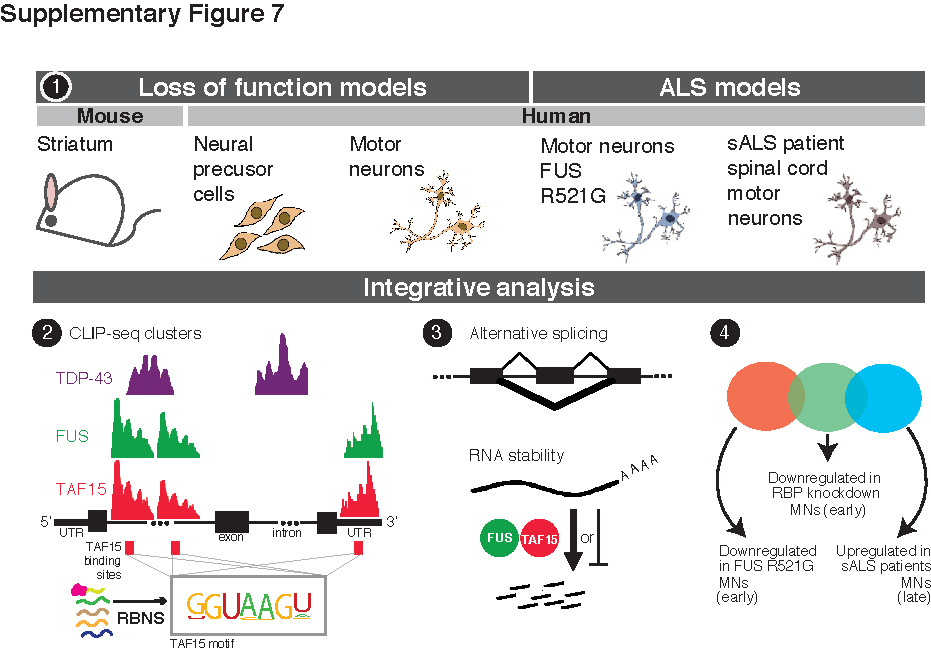
\includegraphics[width=0.5\textwidth]{chapter_3_figures/Figure_S7}
  \caption[Supplementary Figure 6. Considerations for design of splicing maps]{(A) Schematic of overlapping splicing event removal. For all events that overlap with their upstream and downstream exon, the event with the largest percent spliced in (PSI) is chosen as the canonical event. (B) Box plot shows the fraction of events per knockdown experiment removed, based on (x-axis) the number of events within an overlapping window as shown in (A). (C) Comparison of splicing maps generated for RBFOX2 knockdown-excluded cassette exons based on peak density (gold) and background subtracted normalized read density (blue) in HepG2. (D) Histogram indicates the distribution of the number of peaks overlapping significant splicing events for each RBP with both ENCODE eCLIP and knockdown RNA-seq datasets. (E-J) Cassette exon splicing maps for RBP hnRNPK in HepG2, showing 50 exonic and 300 intronic nucleotides for the upstream exon 5’ splice site, cassette exon 3’ and 5’ splice sites, and downstream exon 3’ splice site. Binding around knockdown-excluded (blue), included (red), and native (black) events are shown. (E) Lines indicate read density in IP. (F) Read density in input. (G) Background subtraction splicing map. (H) Information content splicing map. (I-J) Splicing maps indicate mean centered normalized background subtraction and information content scores as compared to IP RPM counts for each significant splicing event at two specific locations: (I) 8bp upstream of the 3’ splice site of the cassette exon, and (J) 42bp downstream of the 5’ splice site of the cassette exon. (K) Full version of Fig. 6H, showing average information content normalized read density before outlier removal at hnRNPC knockdown-excluded (light red) and –included (light blue) events and after performing outlier removal for excluded (dark red) and included (dark blue) events in HepG2. (L) Heatmaps show information content normalized read density in the 3’ section of cassette exon events for hnRNPC (HepG2) before (left) and after (right) outlier removal. (M-N) Comparison of whole-read based inclusion (light blue) and exclusion (dark blue) splicing maps versus 5’ end-only based inclusion (light red) and exclusion (dark red) background subtraction normalized maps for (M) U2AF2 (HepG2) and (N) RBFOX2 (HepG2).\index{Figure_S6}}
  \label{fig:Figure_S6}
\end{figure}

\section{CONCLUSION}
The continuing refinement of methods to identify RNA binding protein binding sites enabled large-scale profiling of targets for 350 RBPs by the ENCODE consortium. This compendium of manually quality assessed datasets provided a unique opportunity to develop rigorous quality metrics that can be applied in an automated fashion to assist in determining reliability of eCLIP experiments, both for large-scale efforts as well as individual eCLIP experiments performed by other groups.

\section{METHODS}

\subsection{Sequencing and data generation for eCLIP}
eCLIP experiments were performed as previously described \cite{VanNostrand2016}. Datasets passing manual quality assessment were deposited at the ENCODE Data Coordination Center (http://www.encodeproject.org) (Supplemental Table S2). Datasets that did not pass but were important for this study are deposited at the Gene Expression Omnibus (accession pending).

\subsection{eCLIP data processing and peak calling}
An exact description of the eCLIP processing pipeline can be found on the ENCODE DCC website (https://www.encodeproject.org/documents/dde0b669\-0909\-4f8b\-946d\-3cb9f35a6c52/\@\@download/attachment/eCLIP\_analysisSOP\_v1.P.pdf). Briefly inline barcodes are used to demultiplex datasets, these and unique molecular identifiers (UMIs) are then removed and recorded using custom scripts. Reads are trimmed using cutadapt (version 1.9), and then mapped against a database of repetitive elements (Repbase version 18.05) using STAR (version 2.4). Reads not successfully mapped to repetitive elements are stringently mapped to the human genome (hg19) using STAR. Finally PCR duplicates were removed using a custom PCR duplicate removal script, and clusters were called using CLIPper (version 1.0). Cluster significance was calculated against a paired input dataset, and significant peaks were defined as clusters with a fold-enrichment ≥ 8 over input and p-value ≤ 0.001.

Repetitive element quantification was performed using a customized pipeline to identify unique mapping to retrotransposable and other multi-copy element families (Van Nostrand et al., in preparation).

Unique fragments were defined as the number of PCR duplicate removed fragments mapping uniquely to the human genome or to a repetitive element family. Unique genomic fragments were defined as the number of PCR duplicate removed fragments uniquely mapping to the human genome. PCR duplication rate was estimated as the fraction of unique fragments to mapped fragments.

For analysis of untrimmed datasets, reads were demultiplexed exactly as described in the eCLIP standard operating procedure, they were then mapped directly to the human genome without any additional processing steps. Percent mapped was reported via STAR mapping output.

For analyses with repetitive elements kept, adapter trimming was performed as normal. Instead of mapping against (and discarding reads mapping to) the database of repetitive elements, reads were immediately mapped to the human genome, and peak calling were performed as previously described. Input normalization was performed using a paired input dataset that also contained repetitive element reads.

For analyses with PCR duplicates kept, all processing, up to PCR duplicate removal was performed as previously described to obtain mapped genomic fragments.  Those fragments were then visualized.

\subsection{Identification of biologically reproducing peaks by IDR}
Peaks reproducing across biological replicates were identified by a modification of the Irreproducible Discovery Rate method \cite{Li2011a} (Supplemental Fig. S2B). Information content for each peak was calculated as $I=p_i*\log_2(\frac{p_i}{q_i})$, with $p_i$ and $q_i$ represent the fraction of total reads in IP and input respectively that map within peak i. Peaks were then ranked by information content, and processed with the IDR software (version 2.0.2) to identify reproducible regions at an IDR threshold of $<$= 0.01. Next, CLIPper-identified clusters within these reproducible regions were queried against both replicates to calculate fold-enrichment and significance in IP versus input. Clusters were ranked by the geometric mean of fold-enrichment between replicates, and a final set of reproducible peaks was identified as the set of non-overlapping CLIPper-identified peaks meeting standard enrichment cutoffs (fold-enrichment $>$=8 and p-value $<$= 0.001) that were highest ranked by fold-enrichment within each reproducible region.

\subsection{Estimation of unique fragments with a-eCT}
PCR amplification can be modeled as $F=I*e^{CT}$, for the number of final molecules yielded $F$, the number of initial molecules $I$, the number of performed PCR cycles $CT$, and PCR efficiency per amplification cycle $e$. Library yield for eCLIP was initially described as an estimated CT (eCT) required to obtain 100 femtomoles of library approximating e = 2:
$eCT=CT-\log_2(\frac{C_{fm}}{100_{fm}})$ for measured library yield C (in femtomoles)(Van Nostrand et al. 2016). Concentrations, PCR Cycle numbers and eCTs for all experiments used in this study can be found in Supplemental Table S2.  Concentrations, PCR cycle numbers and eCTs for control IgG experiments were obtained from (Van Nostrand et al. 2017a).

To obtain an empirical estimate for e, experiments with a PCR duplication rate of $>$90\% were selected. Then a non-linear least squares curve fitting approach was applied to identify the e that minimized the sum of squared error between estimated and observed fragments yielding $\hat{e}$ = 1.84. Accurate-eCT (a-eCT) was the defined as: $aeCT=CT-\log_{1.84}(\frac{C_{fm}}{100_{fm}})$

Calculation of mean squared error was performed by comparing the a-eCT-estimated versus observed number unique fragments in each sequencing experiment.

\subsection{Peak identification dependence on sequencing depth}
The relationship between peak detection and sequencing depth was analyzed by creating pseudo-datasets by subsampling defined fractions of unique genomic fragments. A downsampled series was created by subsampling 10\% of reads, and then iteratively adding 10\% additional reads until all reads were used. Standard CLIPper cluster identification and input normalized peak identification was performed on each downsampled dataset using the same (fully sequenced) input control. Next, each significantly enriched peak identified in the full dataset was associated with the smallest downsampling fraction it was discovered in.
The minimum sequencing depth needed to detect peaks in genes with a given TPM was defined as the number of unique genomic fragments in the downsampled dataset the peak was first discovered in. K562 and HepG2 total RNA TPM values were obtained from ENCODE project accession numbers ENCFF286GLL and ENCFF533XPJ respectively

To consider the correlation between gene expression and number of reads in peaks for eCLIP, the number of reads in each peak was quantified and normalized by peak length. For each gene only the peak with the largest number of reads was selected as representative, and other peaks not considered, to avoid over-weighting large or highly-bound genes. Linear regression comparing the $log_{10}(TPM)$ of the gene to the $log_{10}(normalized read count)$ of the most highly expressed peak was then calculated.

\subsection{Motif or region presence near eCLIP peaks}
To estimate specificity of peaks identified in the downsample series, motif presence (for RBFOX2) and peak location (for PRPF8) were considered. For RBFOX2, a peak was considered as containing a RBFOX2 motif if it overlapped a GCAUG 5-mer on the same strand as the transcript. For PRPF8, a peak was considered properly located if it overlapped the 3’ ends of an exon in GENCODE (v19) (Harrow et al. 2012). For each fraction downsampled, the peaks initially discovered in that fraction were overlapped with the feature of interest to calculate specificity.

To consider sequence conservation within eCLIP peaks, the mean (mammalian) phastcons score was calculated for each peak. Then peaks were grouped by fraction discovered, and the mean conservation of each fraction was calculated. To estimate background conservation, peak locations were shuffled while preserving the number of peaks found in 5’ UTRs, CDS, 3’ UTRs, exons, proximal introns and distal introns, and the mean conservation was calculated. For all RBFOX2 and PRPF8 analysis, downsampling and peak analysis was performed 10 times.

\subsection{Peak and information content saturation analysis}
For saturation analysis, peaks were taken from the above downsampling series. For each downsampling experiment, the fraction of all peaks or fraction of total information content discovered up until the current fraction was calculated. Where total information content is defined as the sum of the information content across all significant peaks.

Saturation was calculated using the equation $\frac{(N_{i}-N_{(i-i)}}{Total}$, where $N_i$ is the number of peaks or total information content recovered at downsampling fraction $i$. Total is the total number of peaks or total information content in the full dataset.

\subsection{Estimates of required reads}
Experiments were defined as saturating when a 10\% increase in reads used lead to a $<$5\% gain in total information. Because peak calling downsampling was performed on unique genomic fragments, the number of unique fragments needed to saturate each dataset was estimated by calculating the number of fragments downsampled if unique fragments had instead been downsampled.

Experiments were rank ordered by read depth when saturated, and the number of unique fragments in the dataset in the 90th percentile was used to estimate the number of unique fragments needed to allow 90\% of datasets to saturate.

Estimation of read loss due to adapter trimming and mapping
Read loss due to adapter trimming and mapping was modeled by calculating the mean fraction of reads lost during each step. Specifically for mapping the fraction lost was calculated as the fraction of mapped fragments from trimmed fragments.

\subsection{PCR duplication downsampling}
Downsampling was performed as described above, however, pre-PCR duplicate mapped fragments, rather than unique genomic fragments were used. The downsampled files were then removed of PCR duplicates as in the main eCLIP processing pipeline and total reads before and after downsampling were counted.

\subsection{Poisson Modeling of PCR Saturation}
For each dataset the relationship between mapped fragments and unique fragments was modeled as a Poisson distribution. The probably that a single fragment was observed at least once is modeled with the equation $P(\leq1)=1-e^{-\lambda}$. Where $\lambda$ is the mean number of times a molecule is observed. $\lambda$ is defined as $\lambda=\frac{M}{E}$. $M$ is the number of mapped fragments and $E$ is the estimated number of unique fragments, as calculated by the a-eCT equation. To estimate the total number of unique fragments $(U)$ from mapped fragments we parameterize the previous equation obtaining $E(1-e^{(-\frac{M}{E})})=U$.

\subsection{Estimates of required reads to sequence}
Estimation of number of sequenced reads needed to observe the required number of unique fragments was performed by integrating the three previously described read loss models. The final model to estimate usable reads from input reads is defined as $S=-E*\frac{ln(1-(U/E))}{P(a)P(m)}$. Where $S$ is the number of reads to sequence, $E$ is the number of estimated unique fragments in the total experiment, $U$ desired number of unique fragments, and $P(a)$ and $P(m)$ are the probably of retaining reads after adapter trimming or mapping.

The naive sequencing depth model was calculated as described in the main text. Specifically $U=(1-P(a))(1-P(m))(1-P(d))*S$, where $U$ is the number of unique fragments, $S$ is the sequenced reads, and $P(a)$, $P(m)$, and $P(d)$ are the probabilities of losing a read due to adapter trimming, mapping or PCR duplicate removal, respectively.

\subsection{Usable read and total information content cutoff calculations}
An optimal unique fragment cutoff for all experiments was calculated by optimizing the f-score. Because many deeply sequenced datasets failed manual QC, for model fitting, only experiments $<$ 1,000,000 reads uniquely genomic fragments were used. The minimum unique fragment threshold was calculated by maximizing the f-score when setting a pass/fail threshold on the number of unique fragments.

A threshold for total information content was developed first by calculating each experiment’s total information content as previously described. For training all datasets passing the minimum unique fragment cutoff were used. To identify an optimal total information content cutoff the cutoff was calculated for all values between 0 and the largest total information content in all experiments. The total information content cutoff that maximized the f-score was determined to be the optimal threshold.

Usable read and total information content values for all datasets used to generated these cutoffs can be found in Supplemental Table S3.

\subsection{Rescue and Self-consistency Ratio}
Rescue and Self-consistency Ratios were calculated as in \cite{Landt2012}. To calculate the rescue ratio, unique genomic fragments from both biological replicates were combined, shuffled, and split into two pseudo-biological replicates. Peak calling and input normalization was then performed. Peaks were ranked by information content and IDR was performed to determine reproducible peaks in the pseudo replicates (Np). Additionally IDR was performed on the real replicates and the number of reproducible peaks was counted (Nt). Rescue Ratio was calculated as $\frac{max(N_p,N_t)}{min(N_p,N_t )}$ .

To calculate self-consistency ratio, uniquely mapped reads from each replicate were independently split into two sub replicates. Peak calling and input normalization were then performed on each set of reads. Within each replicate IDR was performed on information content ranked peaks to determine a reproducible set of peaks. The number of reproducible peaks was then counted for replicate 1 (N1) and replicate 2 (N2). Self-consistancy ratio was calculated as $\frac{max(N_1,N_2 )}{min(N_1,N_2)}$

Self-consistency ratio and rescue ratio values for all datasets used in this study can be found in Supplemental Table S3.

\subsection{Identification of Alternatively Spliced Events}
rMATS (version 3.2.1.beta) JunctionCountsOnly files were used to identify alternatively spliced (AS) events. Significant AS events were defined as having a p-value $>$ 0.05, FDR $>$ 0.1 and ΔΨ $>$ 0.05. Elimination of redundant splicing events was performed by identifying groups of overlapping AS events and selecting the event with the highest inclusion junction count (IJC) among the overlapped events using the bedtools (v2.26) command merge (-o collapse -c 4) and pybedtools (v0.7.9). As a background control 2555 (HepG2) and 3148 (K562) unchanging cassette exons, with 0.1 $<$ Ψ $<$ 0.9 in at least half of control RNA-seq datasets were selected.

\subsection{Generation of splicing maps}
RBP splicing maps were generated using one of four different methods.  For every method all information for significant splicing was extracted in windows near the exon/intron boundary; maximally 50nt into each exon and maximally 300nt into each intron. For shorter exons ($<$100 nt) and introns ($<$600nt), information was only counted until the boundary of the neighboring feature.

For peak binding splicing maps the number of peaks overlapping an AS event were simply summed. IP and input density splicing maps were calculated by computing the mean of the eCLIP normalized (reads per million) read densities over each AS event.

For the background subtraction approach for each splicing event, read densities were first normalized across all regions separately for IP and input, in order to equally weigh each event. Per-position input probability densities were then subtracted from IP probability densities to attain position-level enrichment or depletion.

For information content approach each splicing event’s read densities were normalized by dividing the read depth by the total number of reads in a sample separately for IP and input. Per-position entropy probabilities were calculated using the equation $p(ip) * log_2(\frac{p(ip)}{p(input)})$ where $p(ip)$ and $p(input)$ are the per-position read probabilities at a given base.

To calculate mean normalized enrichment scores for background subtraction and information content methods the mean score for each base was first calculated.  Then each individual event score at each base was normalized by the mean at each base.

\subsection{Outlier removal}
Outliers were moved on a base by base basis. For each base the highest (2.5\%) and lowest (2.5\%) values were removed, and results were visualized

\subsection{Alternative splicing map approaches}
For peak coverage splicing maps the per-base peak coverage of each significant AS event (included or excluded upon knockdown) was summed and reported.

5’ end splicing maps were generated as background subtracted, outlier removed splicing maps, with the exception that full read densities were replaced with just the read density at the 5’ end of the R2 read for each read near an AS event.

\subsection{DATA ACCESS}
Data passing ENCODE quality standards are available on the ENCODE DCC (encodedcc.org).  Data not passing quality standards have been submitted to GEO (accession pending).  All datasets used in this study and their locations are listed in Supplemental Table S2.

\section{ACKNOWLEDGMENTS}
The authors would like to thank Cricket Sloan, Jean Davidson, Eurie Hong, and Mike Cherry for assistance with data deposition and distribution to the public. This work was funded by the National Human Genome Research Institute ENCODE Project, contract U54HG007005, to GWY. ELVN is a Merck Fellow of the Damon Runyon Cancer Research Foundation [DRG-2172-13] and is supported by a K99 grant from the NIH [HG009530]. GAP is supported by the NSF graduate research fellowship. GWY was partially supported by grants from the NIH (HG007005, NS075449).

\section{DISCLOSURE DECLARATION}
E.L.V.N. and G.W.Y. are co-founders and consultants for Eclipse BioInnovations Inc. The terms of this arrangement have been reviewed and approved by the University of California, San Diego in accordance with its conflict of interest policies.
